%% Copernicus Publications Manuscript Preparation Template for LaTeX Submissions
%% ---------------------------------
%% This template should be used for copernicus.cls
%% The class file and some style files are bundled in the Copernicus Latex Package, which can be downloaded from the different journal webpages.
%% For further assistance please contact Copernicus Publications at: production@copernicus.org
%% https://publications.copernicus.org/for_authors/manuscript_preparation.html


%% Please use the following documentclass and journal abbreviations for discussion papers and final revised papers.

%% 2-column papers and discussion papers
\documentclass[journal abbreviation, manuscript]{copernicus}



%% Journal abbreviations (please use the same for discussion papers and final revised papers)


% Advances in Geosciences (adgeo)
% Advances in Radio Science (ars)
% Advances in Science and Research (asr)
% Advances in Statistical Climatology, Meteorology and Oceanography (ascmo)
% Annales Geophysicae (angeo)
% Archives Animal Breeding (aab)
% ASTRA Proceedings (ap)
% Atmospheric Chemistry and Physics (acp)
% Atmospheric Measurement Techniques (amt)
% Biogeosciences (bg)
% Climate of the Past (cp)
% DEUQUA Special Publications (deuquasp)
% Drinking Water Engineering and Science (dwes)
% Earth Surface Dynamics (esurf)
% Earth System Dynamics (esd)
% Earth System Science Data (essd)
% E&G Quaternary Science Journal (egqsj)
% European Journal of Mineralogy (ejm)
% Fossil Record (fr)
% Geochronology (gchron)
% Geographica Helvetica (gh)
% Geoscience Communication (gc)
% Geoscientific Instrumentation, Methods and Data Systems (gi)
% Geoscientific Model Development (gmd)
% History of Geo- and Space Sciences (hgss)
% Hydrology and Earth System Sciences (hess)
% Journal of Micropalaeontology (jm)
% Journal of Sensors and Sensor Systems (jsss)
% Magnetic Resonance (mr)
% Mechanical Sciences (ms)
% Natural Hazards and Earth System Sciences (nhess)
% Nonlinear Processes in Geophysics (npg)
% Ocean Science (os)
% Primate Biology (pb)
% Proceedings of the International Association of Hydrological Sciences (piahs)
% Scientific Drilling (sd)
% SOIL (soil)
% Solid Earth (se)
% The Cryosphere (tc)
% Weather and Climate Dynamics (wcd)
% Web Ecology (we)
% Wind Energy Science (wes)


%% \usepackage commands included in the copernicus.cls:
%\usepackage[german, english]{babel}
%\usepackage{tabularx}
%\usepackage{cancel}
%\usepackage{multirow}
%\usepackage{supertabular}
%\usepackage{algorithmic}
%\usepackage{algorithm}
%\usepackage{amsthm}
%\usepackage{float}
%\usepackage{subfig}
%\usepackage{rotating}


\begin{document}

\title{Radar coherence and NDVI ratios as landslide early warning indicators}


% \Author[affil]{given_name}{surname}

\Author[1]{Mylène}{Jacquemart}
\Author[1]{Kristy}{Tiampo}
%\Author[]{}{}

\affil[1]{Cooperative Institute for Research in Environmental Sciences (CIRES), University of Colorado, Boulder}
%\affil[]{ADDRESS}

%% The [] brackets identify the author with the corresponding affiliation. 1, 2, 3, etc. should be inserted.

%% If an author is deceased, please mark the respective author name(s) with a dagger, e.g. "\Author[2,$\dag$]{Anton}{Aman}", and add a further "\affil[$\dag$]{deceased, 1 July 2019}".

%% If authors contributed equally, please mark the respective author names with an asterisk, e.g. "\Author[2,*]{Anton}{Aman}" and "\Author[3,*]{Bradley}{Bman}" and add a further affiliation: "\affil[*]{These authors contributed equally to this work.}".


\correspondence{Mylène Jacquemart (mylene.jacquemart@colorado.edu)}

\runningtitle{TEXT}

\runningauthor{TEXT}





\received{}
\pubdiscuss{} %% only important for two-stage journals
\revised{}
\accepted{}
\published{}

%% These dates will be inserted by Copernicus Publications during the typesetting process.


\firstpage{1}

\maketitle



\begin{abstract}
The catastrophic failure of the Mud Creek landslide on California's Big Sur Coast on 20 May 2017 highlighted once again how difficult it is to detect a landslide's transition from slow moving to catastrophically unstable. Automatic detection methods that rely on InSAR displacement measurements to detect precursory acceleration are available but can be plagued by imaging geometry complexities and tedious processing algorithms. Here, we present a novel approach for assessing landslide stability by using relative interferometric coherence from Sentinel-1 and Normalized Difference Vegetation Index (NDVI) from Sentinel-2. Our method computes the ratio of mean interferometric coherence or NDVI on the unstable slope relative to that of the surrounding hillslope. We show that the coherence ratio of the Mud Creek landslide dropped by 50\% when the slide began to accelerate five months prior to its catastrophic failure in 2017. Coincidentally, the NDVI ratio began a near-linear decline. In contrast, the landslide accelerated during the rainy seasons of 2015 and 2016, but neither of those accelerations resulted in a drop of the radar coherence ratio. This suggests that radar coherence and NDVI ratios may be able to aid in both the early detection of landslides and indicate whether an acceleration critically threatens the stability of a slope. 
\end{abstract}


\copyrightstatement{TEXT}


\introduction  %% \introduction[modified heading if necessary]
Rainfall triggered landslides are some of the most costly natural hazards worldwide, causing economic loss through damage to infrastructure and livelihoods every year \citep{Petley2012}. To date, our predictions of \textit{where} rainfall triggered landslides are likely to occur mostly rely on regional-to-global scale landslide susceptibility maps \citep{stanley2017}. Predicting \textit{when} a slope is expected to fail is a comparatively harder problem \citep{Intrieri2019}. The most reliable and common approaches for predicting landslides' time of failure all rely on measurements of slope displacements and derivatives thereof (e.g., inverse velocity; \cite{fukuzono1985}). With the exception of open-pit mining, where state-of-the-art monitoring equipment is common and often operates continuously, dense displacement time series of landslides are still the rare \citep{Intrieri2019}. Presently, Norway employs the most extensive landslide detection and monitoring system by continually processing radar data from Sentinel 1-A and 1-B data  \citep{Lauknes2010, dehls2014}. However, generating robust displacement time series from interferometric synthetic aperture radar (InSAR) data is not without challenge due to imaging geometry complexities and tedious processing algorithms. \par 

 More commonly, landslides are mapped after they occur. This practice is particularly important for organizing rescue efforts in response to large numbers of landslides triggered by earthquakes or tropical storms. To this end, landslides are frequently mapped by hand from high-resolution optical images (i.e., \cite{roback2018}), a process that is tedious and time consuming. To speed up the production of such landslide inventories, automated and semi-automated procedures have also developed \citep{mondini2011}. Because landslides frequently damage the vegetation cover, many of the (semi-)automated methods draw on the Normalized Difference Vegetation Index (NDVI; \cite{tucker1979, Rosenthal1985}), which can be calculated from red and near-infrared bands of multispectral optical images.  \par
 
The obvious drawback of approaches that rely on optical imagery is the need for cloud-free imagery, which may not be available immediately after a landslide triggering event (particularly if it was rainfall induced). In contrast, synthetic aperture radar (SAR) has the capability to see through clouds. Due to the increased availability of SAR data (e.g., freely available Sentinel-1 imagery from the European Space Agency), radar-coherence based techniques have recently been explored for the purpose of mapping landslides and damage to infrastructure \citep{Burrows2019, Yun2015}. Radar coherence is a measure of the similarity of a target's scattering properties between two radar acquisitions \citep{zebker1992}. For InSAR applications, where displacements are calculated based on changes of the radar phase, coherence is the primary indicator of data quality. A reduction in radar coherence indicates that either the surface properties of the target have changed or that the imaging geometry has shifted substantially. Because imaging geometries for overlapping Sentinel-1 scenes are generally highly stable, coherence changes are predominantly temporal in nature, making radar coherence a good measure for detecting changes at the Earth's surface. Coherence based landslide mapping has been achieved by classifying a coherence map based on either an absolute coherence threshold, the difference between a pre-event and a co-event coherence map, or the difference between a co-event and a post-event coherence map \citep{Burrows2019, Yun2015}. \par 

InSAR has also been applied to detect precursory acceleration of the 20 May 2017 Mud Creek landslide in California. \cite{Handwerger2019} showed that the seasonal accelerations of the Mud Creek landslide could be tracked throughout the period for which radar data is available, and that a larger speed-up occurred in the months prior to the failure. An acceleration of a landslide body is considered the best indicator for a future failure; however, determining how much acceleration is indicative of impending failure remains unknown. As with the Mud Creek landslide, unstable slopes frequently accelerate seasonally, or in response to temperature changes or precipitation, without failing catastrophically \citep{iverson2000, Segui2020, Handwerger2013}. \par Here, we introduce two novel measures for assessing landslide stability: Radar coherence and NDVI ratio. We evaluate the value of these  measures to provide information about the impending failure of the Mud Creek landslide.

\section{Study site}
The Santa Lucia Mountains rise abruptly from the Pacific Ocean on California's Big Sur Coast, about 150 miles south of San Francisco. Formed in a transpression zone of the San Gregorio-Hosgri Fault System known as the Big Sur Bend, the crest of this rugged, high-relief mountain range rises to over 1700 m asl and is never more than 18\,km from the coast \citep{Johnson2018}. Geologically, Miocene marine sediments,  Mesozoic to Precambrian granitic and metamorphic rocks, as well as Cretaceous-Jurassic marine sedimentary and metasedimentary rocks make up the Santa Lucia Mountains \citep{Graham1978}. The Franciscan Mélange that dominates the geology near Mud Creek consists of mesozoic graywacke sandstones, highly sheared argillite shales, metamorphosed greenstones, and conglomerates, and is well known for its highly variable, but generally low, rock strength \citep{Medley2011, cgs2020}. The Mélange is overlain by unconsolidated, clay rich regolith. \par 
The Big Sur region lies in a Mediterranean climate, where yearly precipitation averages around 1\,$m yr^{-1}$ and typically falls between November and April. The total yearly precipitation depends strongly on the storm and drought cycles controlled by the El Niño Southern Oscillation (ENSO). Following a multi-year drought, the winter of 2016/2017 brought an extraordinary number of intense atmospheric-river driven storms to California, resulting in the state's wettest year on record \citep{swain2018}. 
\par The Mud Creek slide occurred on 20 May 2017, after two weeks with minimal rain. It destroyed almost half a mile of Highway 1, a vital transportation corridor for both tourism and local residents and the only direct connection between Carmel Highlands on the north end of Big Sur and San Simeon to the south. The landslide potential of this particular stretch of road became apparent only in the months preceding the slide, as accumulating debris on the road began to require near daily maintenance \citep{Warrick2019}. Upon recognizing the threat of an imminent landslide, the California Department of Transportation (CalTrans) evacuated all personnel and construction material from the site. Following the catastrophic failure, CalTrans commenced a \$54 million project to construct a new road over the landslide deposit. The highway was reopened on 18 July 2018, more than a year after the slide.\par



\begin{figure}[hbt!]
    \centering
    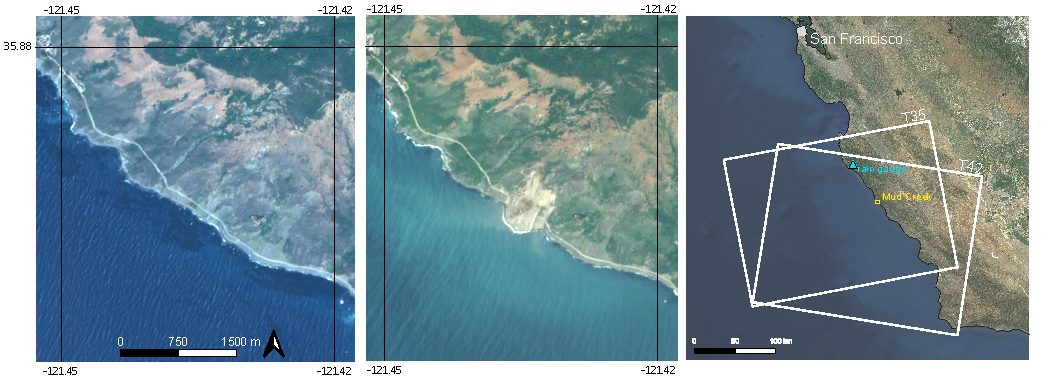
\includegraphics[width = \textwidth]{OverviewFigure_3.pdf}
    \caption{Big Sur coast with Highway 1 before and after the Mud Creek landslide (left and center, images from Copernicus Sentinel-2), and landslide and rain gauge locations and Sentinel-1 ascending (T35) and descending (T42) orbit footprints (right; basemap from ESRI World Imagery - Source: Esri, Maxar, GeoEye, Earthstar Geographics, CNES/Airbus DS, USDA, USGS, AeroGRID, IGN, and the GIS User Community)}
    \label{fig:figure1}
\end{figure}


\section{Methods}
\subsection{Radar data}
In this study we us SAR data from ESA's Sentinel-1 satellite to perform a traditional InSAR displacement analysis and to compute the coherence radar. SAR images contain measurements of backscatter amplitude and radar phase for each point on the ground. Radar backscatter is the amount of energy reflected back to the sensor from each ground point. It is influenced by the geometry of the target, its surface roughness, and dielectric properties. InSAR uses the change in the phase of radar waves between measurements to quantify changes at the Earth's surface. Two SAR images acquired by the same satellite of a given area at different times can be processed into interferograms: images that represent the phase difference [0,$2\pi$] between the two acquisitions at each point. With knowledge of the radar wavelength, these phase changes can be converted to surface displacements. Because InSAR is sensitive to deformation only in the instrument's line of sight (LOS), three independent measurements are  required to obtain the true 3-D motion of a target. In absence of independent measurement, LOS deformations can be projected onto the downslope direction by assuming that the primary motion of a landslide follows gravity.     
\par  
 Alongside any computed interferogram is a coherence $(\gamma)$ image that serves as the primary quality indicator for InSAR data. It is a measure of how similar the ground properties are at the time of the radar acquisitions \citep{Scott2017}, and is computed from the local phase variance in the interferogram. A loss of coherence can be due to  spatial (e.g., a change of satellite viewing geometry) or temporal changes (e.g., change in surface properties like vegetation growth). On a vegetated slope like Mud Creek, coherence is predominantly controlled by three factors: A change in the dielectric properties of the soil due to a change in soil moisture \citep{molan2020}, changes to the geometric characteristics of the surface due to growth or removal of vegetation (e.g., \cite{Ruescas2010}), or displacement of the target that is larger than half a radar wavelength between two SAR acquisitions \citep{Zhou2009}. \par

For our analyses, we used JPL's InSAR Scientific Computing Environment (ISCE; \cite{rosen2012}) and processed 51 Sentinel-1 images from the ascending orbit (track 35) and 64 from the descending orbit (track 42). SAR images for our study site were available back to April 2015, with images typically acquired every 12 days. We obtained Single Look Complex (SLC) images for tracks 35 (ascending) and 42 (descending) from the Alaska Satellite Facility (ASF DAAC: \url{https://search.asf.alaska.edu/#/}). We allowed for a maximum time difference of 48 days between images and produced 172 interferograms from the ascending orbit and 208 from the descending orbit (see Table \ref{tab:products}). Because of a gap in data availability from the ascending orbit between late 2015 and early 2016, we increased the permissible time difference between images in that period to 6 months. This allowed us to produce a connected network of interferograms for both orbits. We multi-looked the images with two looks in range and one look in azimuth, and removed the topographic phase with a 10\,m DEM obtained from the USGS' National Map Server (\url{https://viewer.nationalmap.gov/basic/}).  

\par Images with low overall coherence are typically omitted from InSAR analyses. Because our area of interest is small relative to the size of the full interferogram, mean image coherence is a poor indicator for the data quality in our area of interest. Rather than manually identifying low quality images, we calculated the mean coherence within our area of interest for each interferogram and only retained images with a mean coherence above a defined threshold. We then computed time series of displacement, radar coherence ratio and amplitude ratio from all the retained images.\par 

\begin{table}[hbt]
    \centering
     \caption{Overview of data products used in this study and the number of products derived at the different processing steps.}
    \begin{tabular}{c| c c c c c}
    Product & Raw images & Cloud-free NDVI images & Interferograms & Ratio processing  & Displacement processing \\ 
    \hline
         Sentinel-2 & 23 & 22& -& 22 & -\\ 
         Sentinel-1 ascending & 35 & - & 172 & 132 & -\\
         Sentinel-1 descending & 42 & - & 208 & 141 & 193
    \end{tabular}
    \label{tab:products}
\end{table}

 \subsubsection{Displacement}
To produce a displacement time series we used only data from the descending track and removed all interferograms with a mean coherence of less than 0.35. This produced a fully connected time series with 193 interferograms. We selected a point just south of the landslide as our stable reference region and computed a time series using the NSBAS method implemented in JPL's Generic InSAR Analysis Toolbox (GIAnT; \cite{agram2013}). We retrieved surface displacements by projecting the measured line of sight deformation at each point onto the fall line. To do this we defined the unit line of sight vector \textit{a} to point from the satellite to the target and the unit fall line \textit{b} to point from target down slope along the steepest gradient. We describe both vectors in a polar coordinate system where $\theta$ describes a positive counter-clockwise rotation from x, and $\phi$ describes the angle from positive up (Fig. \ref{fig:los}). The full slope parallel deformation $D_t$ could then be retrieved as
\begin{equation}
    D_t = \frac{LOS}{cos(\delta)}, 
\end{equation}
where LOS is the measured line of sight deformation and $\delta$ is the angle between \textit{a} and \textit{b}, which is defined as:
\begin{equation}
    cos(\delta) = \frac{a \cdot b}{\rvert a \rvert \rvert b \rvert}
\end{equation}
  
\begin{figure}[hbt!]
    \centering
    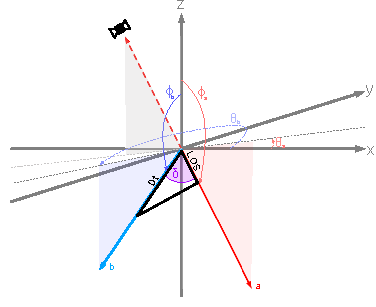
\includegraphics[scale = 1.5]{los_projections.pdf}
    \caption{Vector geometries used to project measured line-of-sight displacements (\textit{LOS}) onto the fall line (\textit{b}). For \textit{a} and \textit{b}, $\theta$ describes the azimuth from x (East) and $\phi$ describes the angle from positive up. The angle $\delta$ between \textit{a} and \textit{b}, controls how much of the true deformation is visible in the satellites LOS.}
    \label{fig:los}
\end{figure}  


\subsubsection{Amplitude and coherence ratios}
To construct a time series of coherence and amplitude evolution, we filtered out all interferograms with mean coherence of less than 0.5 in our area of interest (Fig. \ref{fig:coherence_filter}). This higher threshold was necessary to detect any differences between the unstable part of the slope and the surrounding area. We retained 132 interferograms from the ascending track and 141 interferograms from the descending track after applying this filter criterion.\par 
ISCE computes coherence using a 5 x 5 pixel triangular weighted window. For signals $s_1$ and $s_2$, coherence is given by
\begin{equation}
    \gamma = \frac{\lvert \langle s_1 s^*_2\rangle\rvert}{\sqrt{\langle s_1 s^*_1\rangle \langle s_2 s^*_2\rangle}}\qquad 0\leq | \gamma | \leq 1,
\end{equation}
where * indicates the complex conjugate \citep{jung2016}.\par
We created a time series of radar coherence ratio ($C_R$) by calculating the ratio between the mean coherence over the slide (the area that ultimately failed) and the mean coherence over the surrounding slope (termed Reference Slope, see Figure \ref{fig:coh_evolution}) as:\par
\begin{equation}
    C_R=\frac{\overline{\gamma}_{Slide}}{\overline{\gamma}_{RefSlope}}
\end{equation}
Equivalently, we computed the amplitude time series as
\begin{equation}
    A_R=\frac{\overline{\sigma}^0_{Slide}}{\overline{\sigma}^0_{RefSlope}},
\end{equation}
where $\overline{\gamma}_{Slide}$ and $\overline{\sigma}^0_{Slide}$, and $\overline{\gamma}_{RefSlope}$ and $\overline{\sigma}^0_{RefSlope}$ are the mean values of radar coherence and backscatter over the slide and reference slope, respectively. The reference slope was determined from optical images and a DEM to include the surrounding hillslope with similar aspect and vegetation pattern. Figure \ref{fig:coh_evolution} shows the evolution of the coherence on the slide and surrounding hillslope for four interferograms acquired in the fall of 2016 and spring 2017.  

\begin{figure}
    \centering
    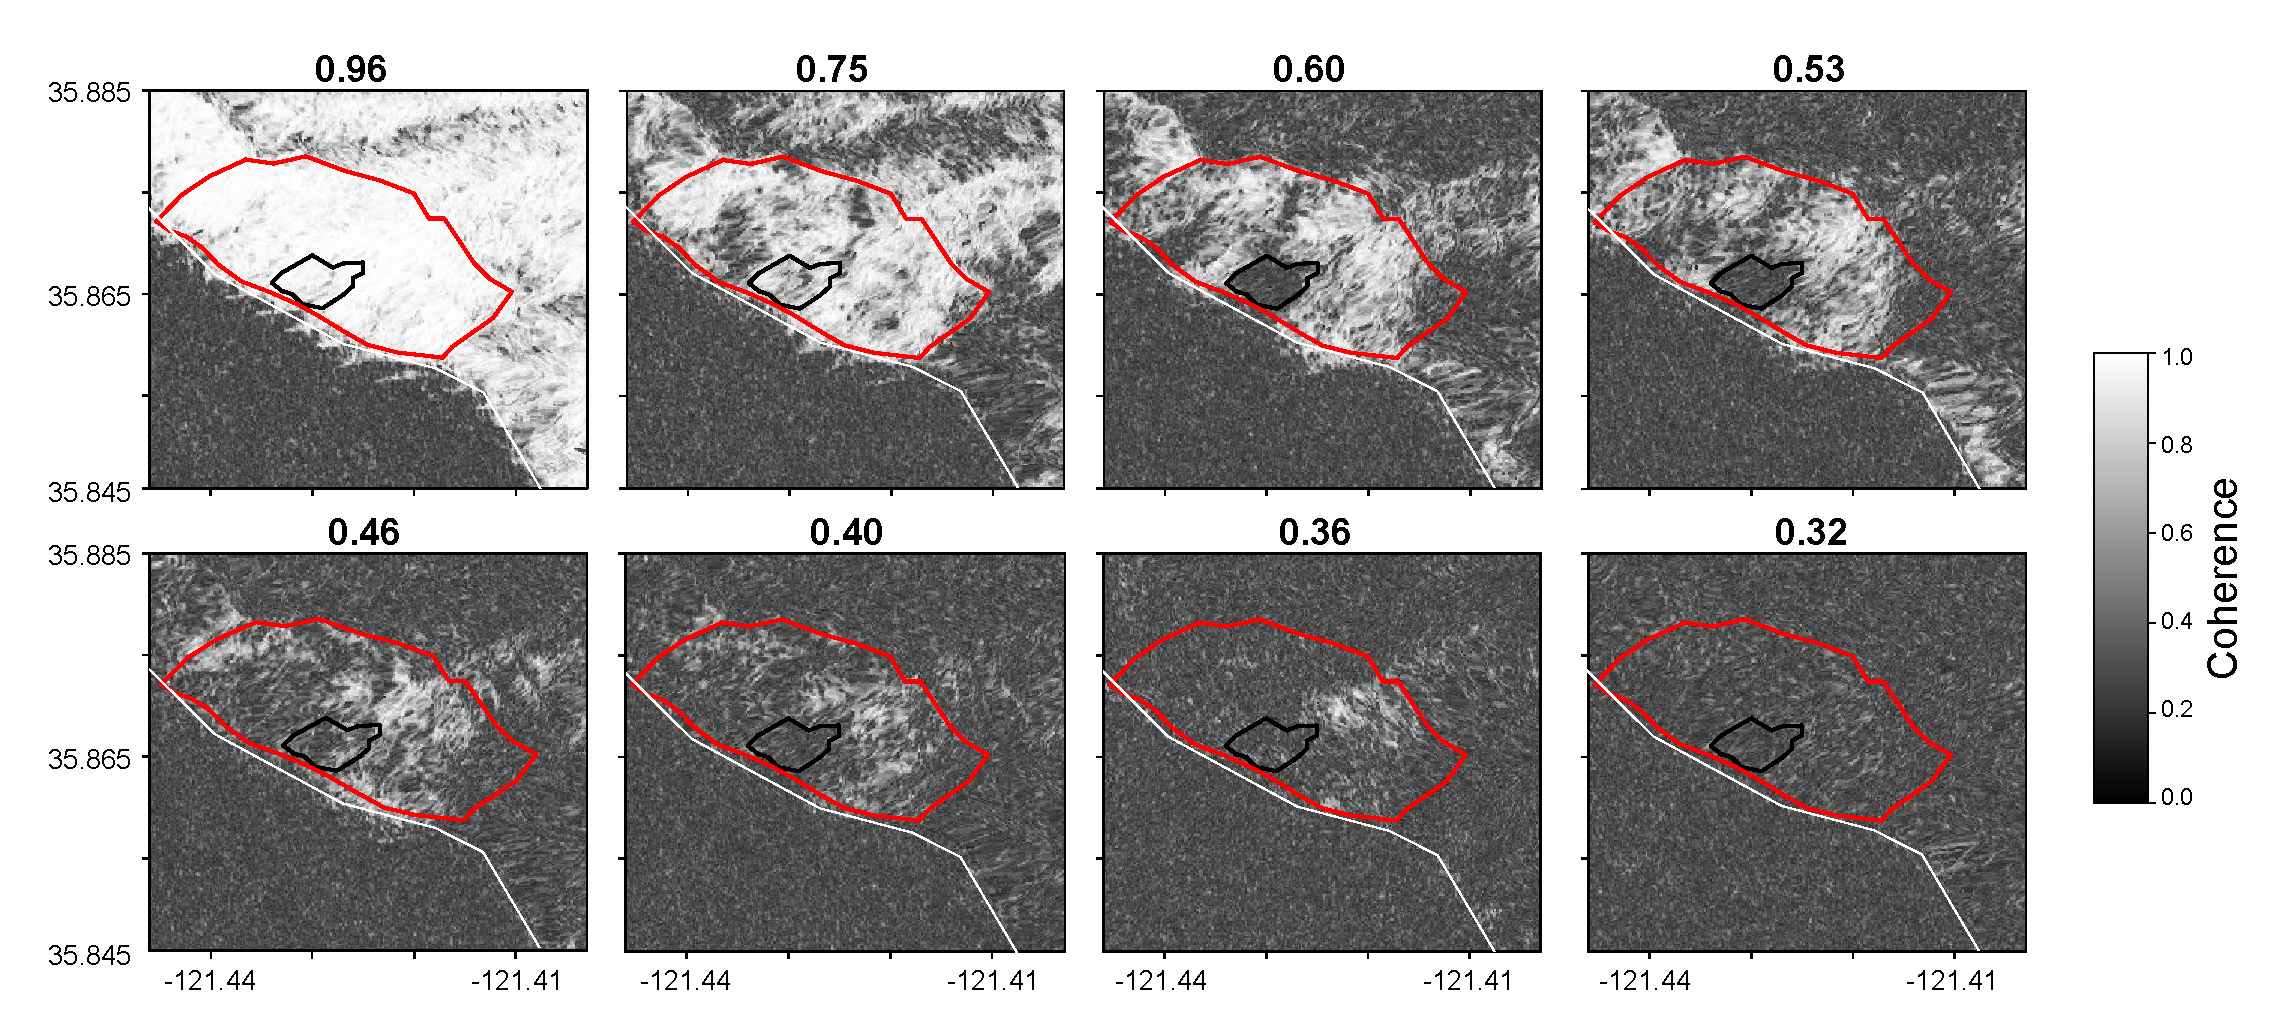
\includegraphics[width = \textwidth]{coherence_filter_sample_bw.pdf}
    \caption{Example of coherence filtering for interferogram selection with a threshold of 0.5 within the area of interest (red polygon). The upper row of interferograms is included to compute the coherence ratio, the lower row is not. The computed mean coherence is given above each panel. The 20 May 2017 landslide occurred inside the black outline (corresponding to dashed gray line in Fig. \ref{fig:displacement}). Coherence derived from Copernicus Sentinel-1 data.}
    \label{fig:coherence_filter}
\end{figure}

\begin{figure}[hbt!]
    \centering
    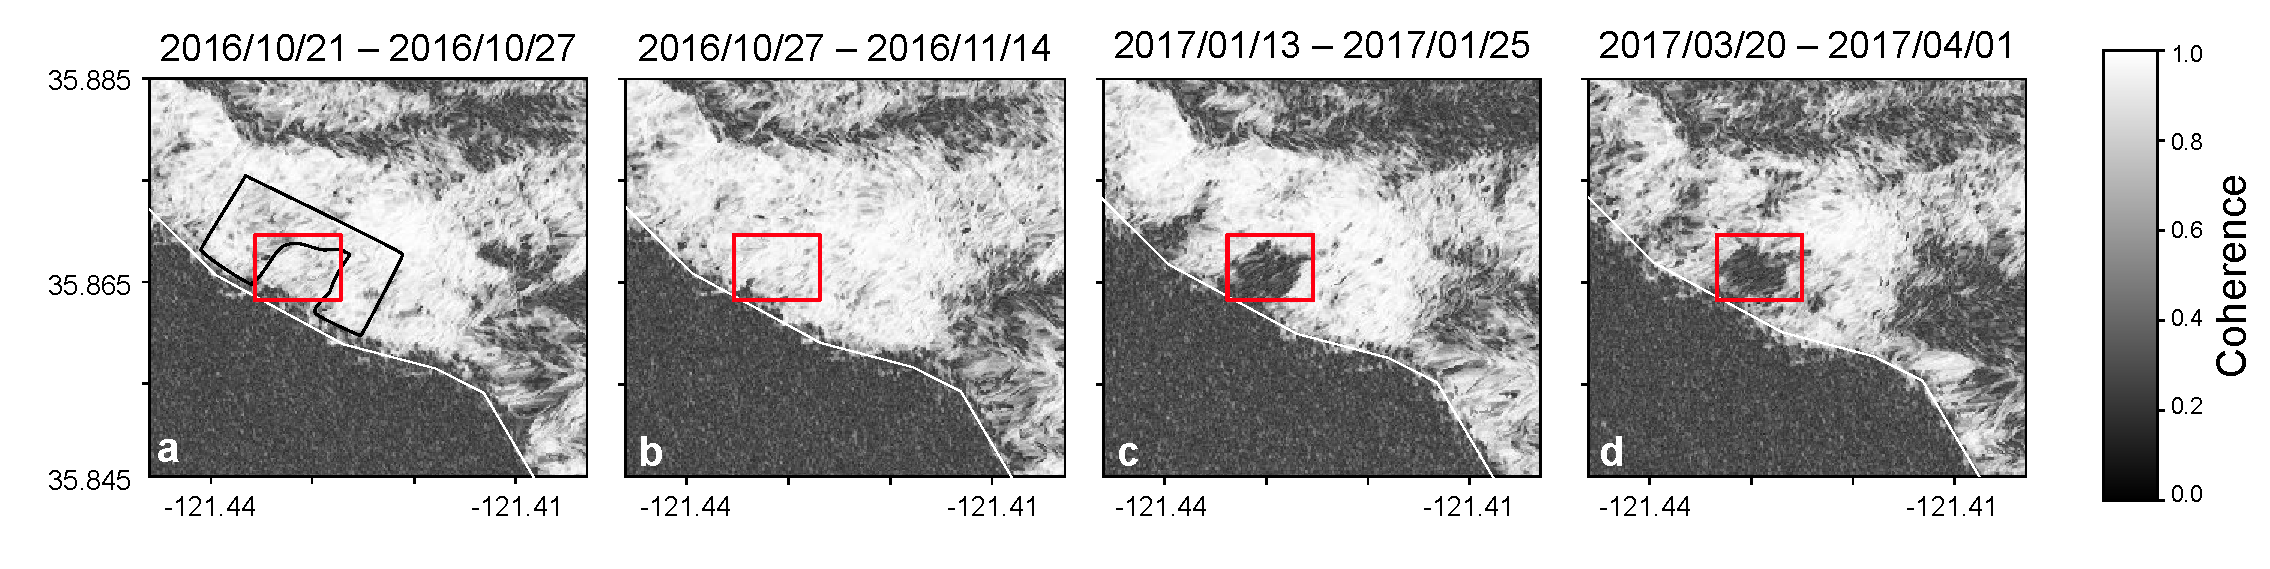
\includegraphics[width = \textwidth]{coherence_evolution_withref.pdf}
    \caption{Interferometric coherence of the Mud Creek landslide and surrounding slope in Fall 2016 (a \& b) and Spring 2017 (c \& d). The coherence loss in the area from which the May 2017 failure originated is framed by the red rectangle. The reference hillslope is outlined in black. Coherence derived from Copernicus Sentinel-1 data.}
    \label{fig:coh_evolution}
\end{figure}

\subsection{Optical data}
To investigate whether coherence changes were driven by changes in vegetation cover, we computed a time series of Normalized Difference Vegetation Index (NDVI), a measure of vegetation productivity that can be derived from optical satellite imagery. NDVI was computed from bands 4 (red) and 8 (near infrared) of ESA's Sentinel-2 (10\,m resolution) as \par

\begin{equation}
    NDVI = \frac{{B8 - B4}}{{B8 + B4}}
\end{equation}

By design, NDVI values vary between -1 and 1, where denser or more productive vegetation results in more positive values and sparse vegetation or bare ground results in low or negative values. We calculated the NDVI for all available cloud-free images back to January 2016 and then computed our time series in the same manner that we did for the amplitude and coherence ratios: \par
\begin{equation}
    NDVI_R= \frac{\overline{NDVI}_{Slide}}{\overline{NDVI}_{RefSlope}}
\end{equation}

\subsection{Precipitation data}
Precipitation data were obtained from the National Oceanic and Atmospheric Administration's (NOAA) Global Historical Climate Network Daily (GHCND) stations. The Big Sur Station station is located 53 km north-west of Mud Creek at 61 m asl.% the Hearst Castle station is located 31 km south-east of Mud Creek at an elevation of 465 m asl. %In order to investigate the spatial precipitation patterns, we acquired NASA IMERG data. We compared IMERG precipitation time series from Mud Creek, Big Sur Station, and Hearst Castle to each other as well as to the GHCDN station data. 

\section{Results}
\subsection{Deformation}
Because InSAR only detects the component of motion in its line of sight, the local incidence angle critically controls how much motion the radar can see. At Mud Creek, the radar's line of sight on the ascending orbit intersects the fall line at a near right angle in most places, impeding the detection of downslope motion. On the descending orbit, the line of sight intersects the fall line at more favorable angles, allowing us to retrieve about 50\% of the total displacement.\par 
Figure \ref{fig:displacement} shows the slope parallel displacement obtained from the descending track. The total cumulative displacement on the Mud Creek landslide since April 2015 (beginning of Sentinel-1 measurements) range from $\sim$0.15\,m to $\sim$0.55\,m. The displacement time series at three different points on the slope all show moderate spring to early summer speed-ups in 2015 and 2016, followed by a large acceleration in 2017. The area showing measurable displacements is somewhat larger than the area that failed on May 20th, but smaller than the area that consistently showed low coherence in the months preceding the landslide (Fig \ref{fig:displacement}).

\begin{figure}[hbt!]
    \centering
    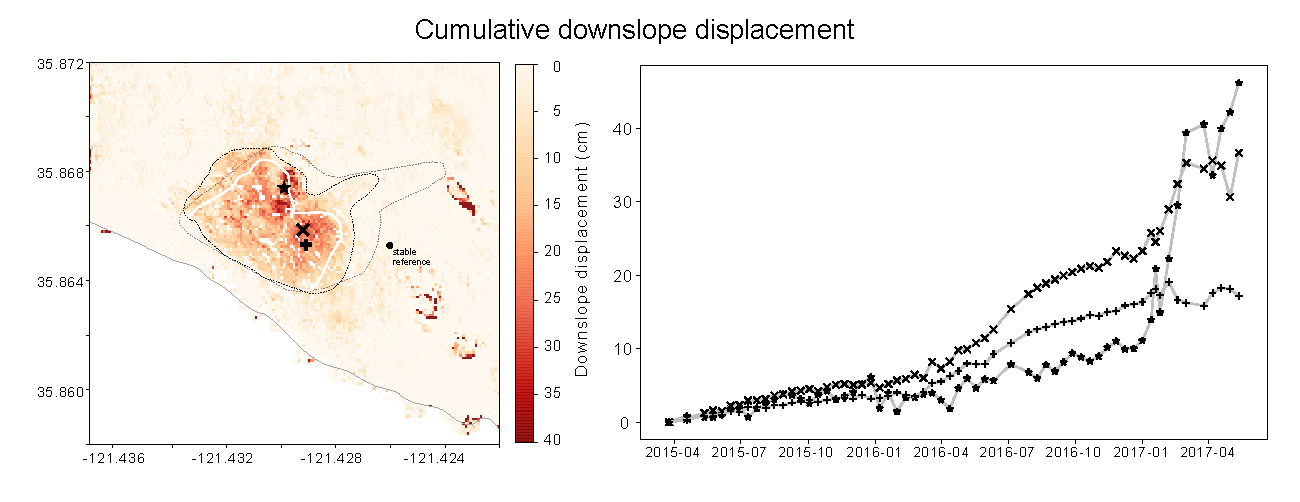
\includegraphics[width=\textwidth]{displacement_all_outlines.pdf}
    \caption{Left: Cumulative line of sight displacements from April 2015 to May 2017 projected onto the fall line. Right: Time series of displacement at three different points within the slide (indicated by the $\bigstar$, $\times$ and + signs). The white line indicates the extent of the slope that failed, the dashed black line the area showing significant displacement, and the dashed grey line the area of low coherence.}
    \label{fig:displacement}
\end{figure}

\subsection{Amplitude \& coherence ratios}
The results of coherence, amplitude, and NDVI ratios are shown in Figures \ref{fig:coherence_timeseries} and \ref{fig:amplitude_timeseries}. The 132 good quality interferograms from the ascending orbit form a mostly-continuous time series, though there was a gap in data acquisition in late 2015 and early 2016. The descending track offers a more continuous time series between 2015 and early 2017, but few interferograms in 2017 passed the coherence threshold. Until early 2017, coherence ratio hovers around 1, indicating that changes in coherence affect both the slide and the reference slope similarly. Then, coincident with the large increases in cumulative precipitation, a stark drop in coherence ratio of around 0.4 (or -50\%) occurs in early 2017.  \par
The amplitude time series on both the ascending and descending tracks show some seasonal trends, but there is no clear difference between 2017 and earlier years. It appears that there is little difference between the backscatter received from the slide body and the surrounding slope in the descending track. Conversely, the backscatter received from the slide body on the ascending track is higher than that of the surrounding slope.  

\begin{figure}[hbt!]
    \centering
    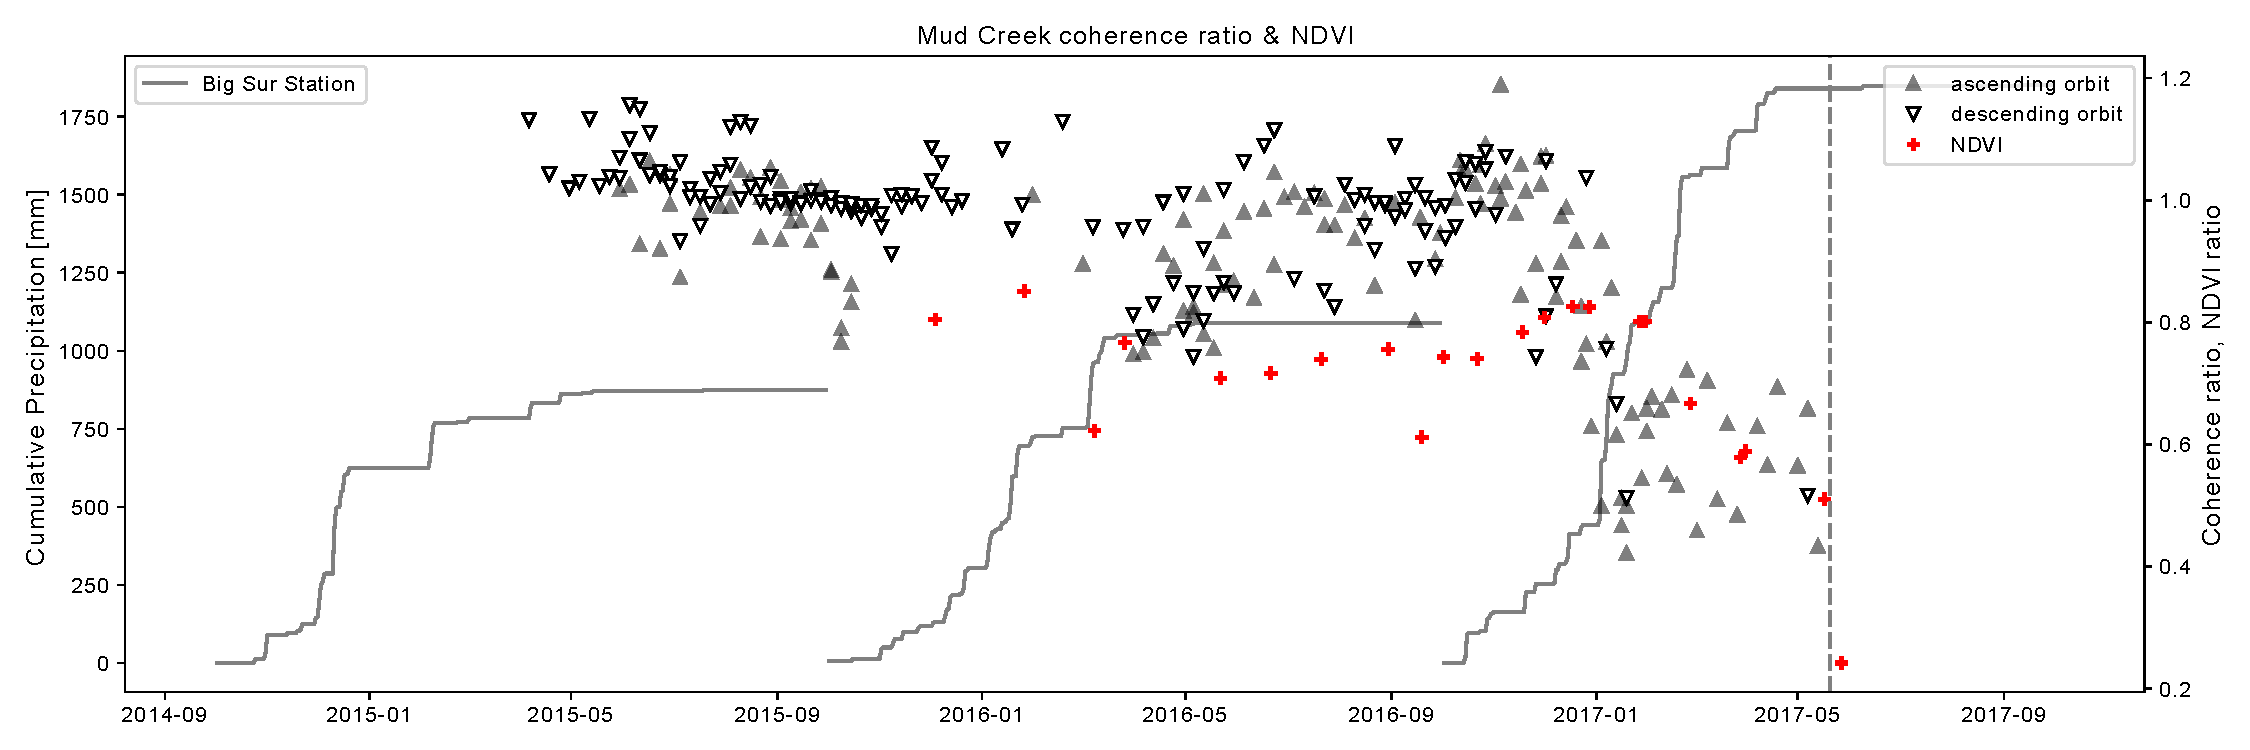
\includegraphics[width = \textwidth]{coherence_ndvi.pdf}
    \caption{Radar \textbf{coherence} ratio plotted against NDVI ratio and cumulative precipitation (at Big Sur Station). The dashed line indicates the timing of the landslide.}
    \label{fig:coherence_timeseries}
\end{figure}

\begin{figure}[hbt!]
    \centering
    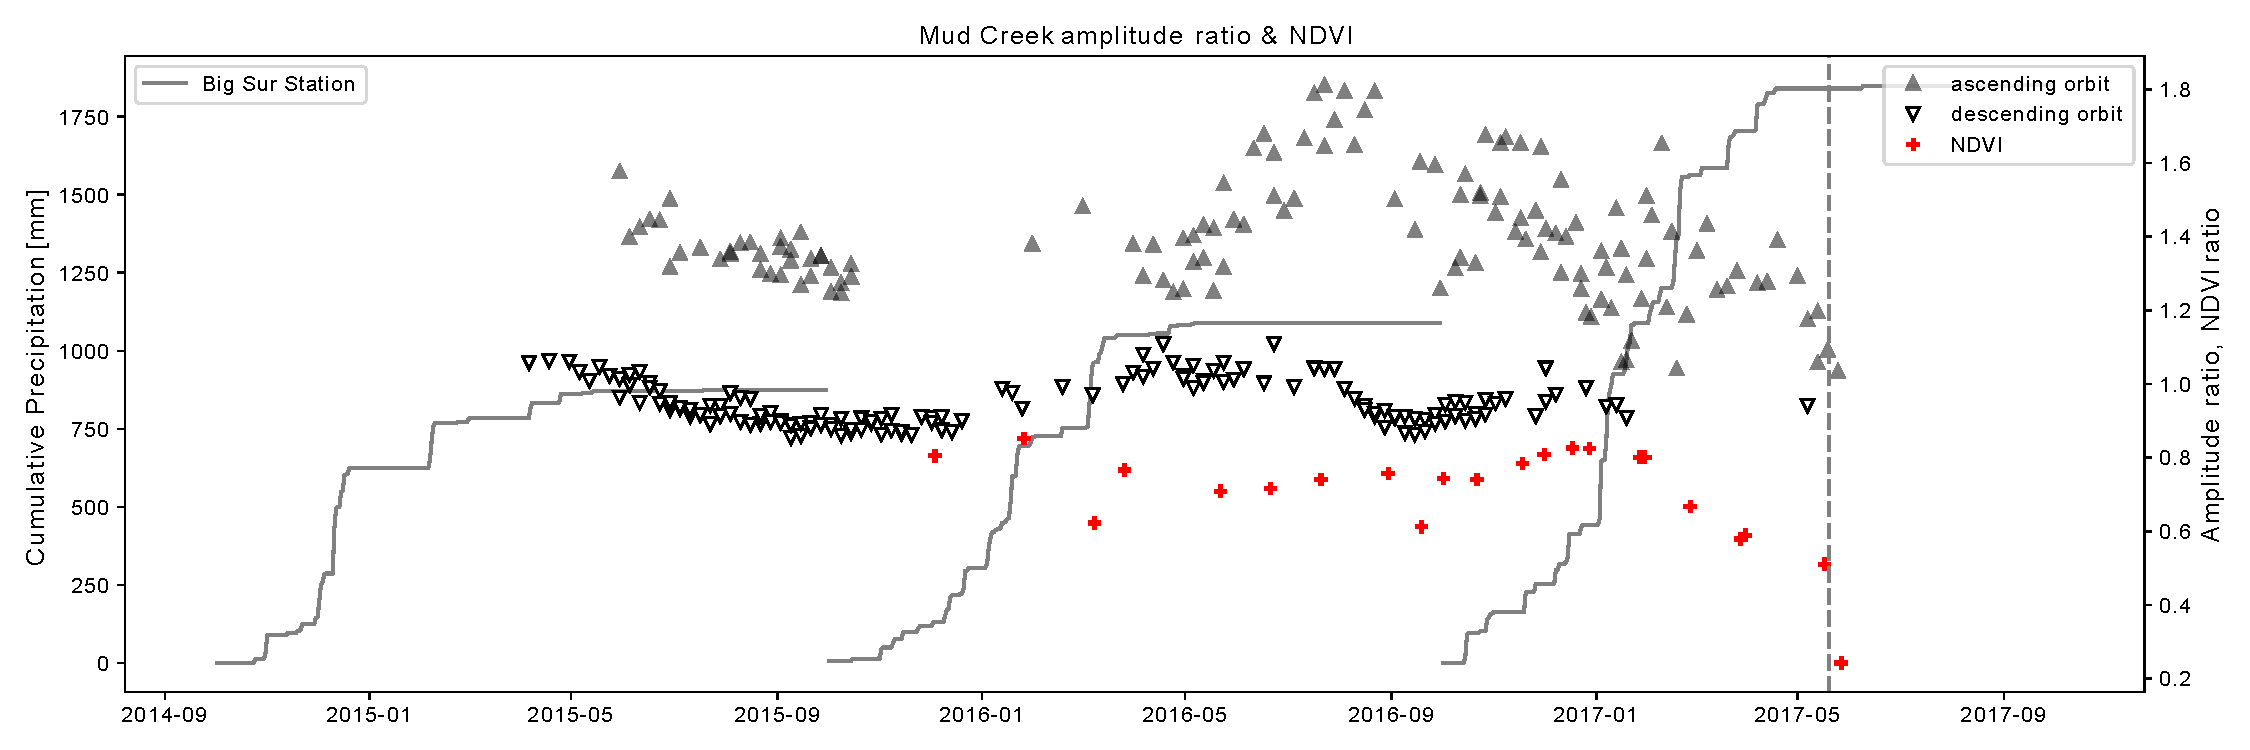
\includegraphics[width = \textwidth]{amplitude_ndvi.pdf}
    \caption{Radar \textbf{amplitude} ratio plotted against NDVI ratio and cumulative precipitation (at Big Sur Station). The dashed line indicates the timing of the landslide.}
    \label{fig:amplitude_timeseries}
\end{figure}

\subsection{NDVI}
The average NDVI ratio of 0.8 prior to 2017 indicates that the Mud Creek slope is generally less densely vegetated than the surrounding hillside. However, starting in early 2017, the gradual decline of the NDVI ratio indicates that vegetation cover within the slide area was degrading. In addition to the ratio time-series, we computed the mean NDVI for the slide area and the reference slope separately to ensure that the evolution of the NDVI ratio is in fact controlled by a decrease of vegetation productivity on the slide and not an increase of productivity on the reference slope (Fig \ref{fig:ndvi_noratio}). These individual time series reveal that the evolution of the vegetation cover on the slide closely paralleled that of the reference slope in 2016, with productivity peaking in April. In early 2017, we observe a clear divergence of the two curves, as vegetation productivity in the slide area began to decline before plummeting post-slide. We also observe a single outlier in April 2016, where the NDVI on the slide exhibited a sudden drop, not seen on the surrounding slope. Incidentally, this drop coincided with the 2016 acceleration reported by \citep{Handwerger2019}.   \par
 
\begin{figure}[hbt!]
    \centering
    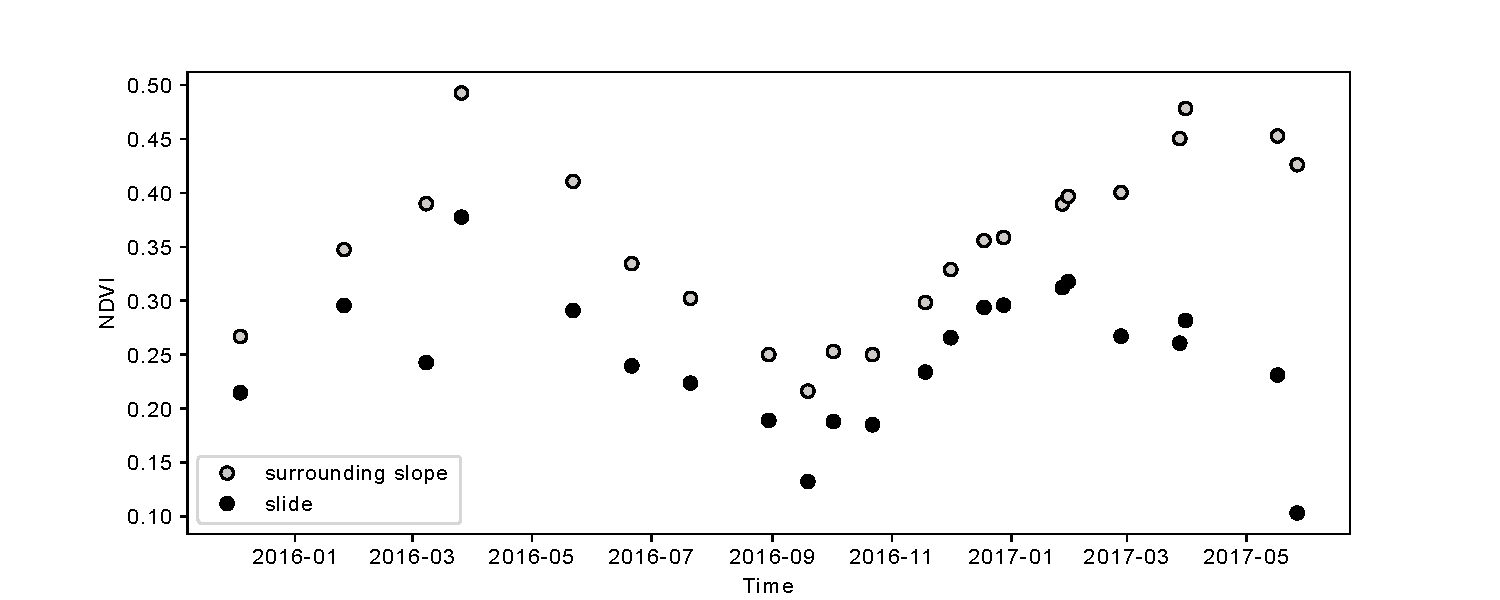
\includegraphics[scale = 0.5]{NDVI_noratio.pdf}
    \caption{NDVI on the Mud Creek slide body and the surrounding slope. Note that the last data point in May 2017 is from an image acquired after the landslide.}
    \label{fig:ndvi_noratio}
\end{figure}


\section{Discussion}
Identifying slopes prone to catastrophic failure, or forecasting when a known landslide will fail, remains a largely unsolved challenge. Five months before its final failure, in conjunction with some of the largest rainfall events measured during California's 2016/2017 winter, the coherence ratio over the Mud Creek landslide dropped by 50\%. At the same time, the NDVI ratio began a near linear decline (see Figure \ref{fig:coherence_timeseries}). These data raise the question of what such observations reveal about the driving processes and/or whether they can be valuable indicators of impending landslides. \par
Even where the location of a landslide is known, reliable predictions of the anticipated failure time have only been achieved in a few cases \citep{Intrieri2019, Loew2016}, and typically require ground-based measurements of displacement rates. As in many cases, the deformation of the Mud Creek landslide was only investigated after the failure \citep{Handwerger2019, handwerger2015}. While this practice provides important insights into landslide mechanics, it does not provide advance warning that can be used to mitigate damage. As \cite{Handwerger2019} show, unwrapping errors make measuring the true surface velocities particularly difficult for fast moving and accelerating landslides. Because radar measurements only reveal phase changes in modulo $2\pi$, a displacement of $\pi$ looks identical to one of $3\pi$. Unwrapping errors can be reduced by subtracting the mean landslide velocity prior to the phase unwrapping. This can reveal the missing phase cycles and help recover more of the true deformation \citep{handwerger2015, Handwerger2019}. However, this approach requires assessing each landslide individually, and does not lend itself to automatic processing at large scales. We did not apply a correction to subtract the mean landslide velocity and are therefore not able to recover the full deformation. In particular, we cannot recover the acceleration in 2016 due to unwrapping errors that mask the true acceleration that year. Nevertheless, our $\sim$0.6\,m cumulative surface displacement measurements are in good agreement with the $\sim$0.8\,m  reported by \cite{Handwerger2019}, and the temporal displacement patters beyond 2016 are nearly identical. Thus acceleration prior to the failure is therefore detectable, even if a landslide velocity model is not applied. This suggests that InSAR-derived surface displacements can be used to identify slope instabilities; however, the significant impact of the unwrapping errors highlight that such an approach is not without challenges and may not yield reliable results. \par
Our time series of coherence ratios indicates that a more systematic analysis of these data might provide valuable information for landslide detection and warning. The premise is that general environmental and atmospheric changes (e.g., vegetation cycles, meteorologic storms, ionospheric disturbances) affecting InSAR coherence should not vary between a landslide and its surrounding slopes. If they do, then we should be able to link that difference to changes on the ground. The observed loss of coherence is likely to be caused by one or more factors influencing coherence: Changes to the dielectric constant of the ground, the local surface geometry, or an acceleration of the slope, and we currently can not parse out the contributions of the different factors in detail. However, we can draw on amplitude, NDVI ratios and displacement to shed some light on the temporal evolution of the coherence ratio: Changes of soil moisture alter the dielectric constant of soil, which can lead to a loss of coherence. Moister soils are typically associated with higher radar backscatter \citep{oldak2003, paloscia2013}. The amplitude time series indicates that average backscatter from the slide body was slightly higher (ascending orbit) or equal (descending orbit) to that of the surrounding slope. However, there is no discernible trend that sets 2017 apart from previous years. We interpret these data to show that the Mud Creek slide may have been slightly wetter than the surrounding slope, but that this difference is not significant, and does not seem to persist into 2017. The NDVI ratio began its near linear decline concurrent with an observed the reduction in the coherence ratio. However, the NDVI decline is gradual, indicating that the change of vegetation cover - and therefore the surface geometry - was not sudden. This observation is supported by the reported, continuous sloughing off of vegetation and debris during spring 2017 \citep{Warrick2019}. The removal of vegetation decreases root cohesion (e.g., \cite{schmidt2001}), promoting additional surface erosion, which would also contribute to an altered surface geometry. Finally, high displacement rates observed in early 2017 can also have contributed to the loss of coherence by surpassing the amount that can be unambiguously determined with InSAR. Combined, these data suggest that, initially, the stark coherence loss may have been driven by the acceleration of the slope in early 2017. Following the initial acceleration, the degradation of the vegetation cover throughout the spring of 2017 may be responsible for and/or have contributed to coherence ratio remaining low until the final failure. \par
The discrepancies between the low coherence area, the area that exhibits measurable surface displacements and the area that ultimately failed indicate that neither displacement nor vegetation degradation can fully explain the low coherence values; since neither of the two changes were observed in these peripheral areas of the low coherence region (Fig. \ref{fig:displacement}). This observation highlights the need to estimate the individual contributions of different factors to the coherence drop, especially their temporal evolution and interplay. 
%In the larger landslide context, the stability of a slope can be expressed in terms of its Factor of Safety (FoS, \cite{Lu2006,Lu2012}), which describes the ratio between shear strength and shear stress on a slope. A FoS <1 indicates an unstable configuration with a higher shear stress than shear strength. We interpret the low radar coherence in conjunction with the decreasing NDVI values to indicate that, at a minimum, the near-surface part of the Mud Creek slope became unstable in January of 2017, five months prior to the failure. \par
 %With a coherence threshold of 0.5, few descending images from 2017 pass the quality threshold, while most from the ascending track do. The coherence filtering removed 23\% of all interferograms from the ascending track, and 32\% of all interferograms from the descending track. During the critical acceleration period in 2017, 14% of interferograms from the ascending track were filtered out, and 18% from the descending track.  %We do not currently have an explanation for this difference. We hypothesize that the near normal (in the geometric sense) incidence angle from the ascending track causes less scattering on vegetation that its more oblique counterpart from the descending track. This effect generally reduced the coherence in the descending track, even on the reference slope, making those data unsuitable for the calculation of coherence ratio. 
 %This observation also raises the question as to what the ideal filtering threshold is. In this case, we opted for sticking with the same threshold for both datasets, rather than adjusting the threshold based on the data. Further analyses on different landslides will help determine the adequate value for this parameter.
\par
A main disadvantage of relying on surface displacements remains the viewing geometry. As in the the case of the ascending track at Mud Creek, unsuitable viewing geometries can significantly impede displacement measurements. In contrast, we note that the coherence data from the ascending track - the track that is not well suited to measure surface displacements - provide the more continuous time series of coherence ratio during the spring 2017 acceleration. Therefore, a systematic analysis of radar coherence may complement traditional InSAR measurements in valuable ways. The radar coherence ratio remained steady during the acceleration phases in 2015 and 2016 which were followed by renewed stabilization of the slide. In 2017, during the acceleration period that preceded catastrophic failure, the coherence ratio experienced a step decrease five months prior to failure, while the NDVI ratio showed a linear decline; it is unclear whether the momentary NDVI drop in 2016 was due to the slope acceleration that year. It is evident that NDVI ratios are limited to vegetated slopes, and a more in-depth analysis of NDVI ratio and coherence ratio at multiple landslide sites is necessary to assess their full value. Nonetheless, both the coherence and NDVI approach are simple to compute and could be applied at large scales. Such techniques would be especially beneficial in areas where InSAR-derived pre-failure acceleration is difficult to resolve.  \par


\par
% \cite{damageassessment}. In this way, landslides are frequently mapped after they happened. 
% The 



\conclusions  %% \conclusions[modified heading if necessary]
Radar coherence has long been used to assess areas of damage after natural catastrophes, but the value of radar coherence as a possible predictor for impending landslides has not yet been studied. In this study we showed that time series of radar coherence ratio and NDVI ratio may be able to distinguish a non critical acceleration of a landslide from one leading to failure many months in advance. Comparatively easy to compute, radar coherence ratios have the potential to be generated at large spatial scales to identify unstable slopes. We believe that the encouraging initial results presented here motivate further investigations of these new parameters.

%% The following commands are for the statements about the availability of data sets and/or software code corresponding to the manuscript.
%% It is strongly recommended to make use of these sections in case data sets and/or software code have been part of your research the article is based on.

\codeavailability{https://github.com/mjacqu/MudCreek} %% use this section when having only software code available


%\dataavailability{TEXT} %% use this section when having only data sets available


%\codedataavailability{TEXT} %% use this section when having data sets and software code available


%\sampleavailability{TEXT} %% use this section when having geoscientific samples available


%\videosupplement{TEXT} %% use this section when having video supplements available


%\appendix
%\section{}    %% Appendix A

%\subsection{}     %% Appendix A1, A2, etc.


%\noappendix       %% use this to mark the end of the appendix section. Otherwise the figures might be numbered incorrectly (e.g. 10 instead of 1).

%% Regarding figures and tables in appendices, the following two options are possible depending on your general handling of figures and tables in the manuscript environment:

%% Option 1: If you sorted all figures and tables into the sections of the text, please also sort the appendix figures and appendix tables into the respective appendix sections.
%% They will be correctly named automatically.

%% Option 2: If you put all figures after the reference list, please insert appendix tables and figures after the normal tables and figures.
%% To rename them correctly to A1, A2, etc., please add the following commands in front of them:

%\appendixfigures  %% needs to be added in front of appendix figures

%\appendixtables   %% needs to be added in front of appendix tables

%% Please add \clearpage between each table and/or figure. Further guidelines on figures and tables can be found below.



\authorcontribution{Mylène Jacquemart designed the study, processed and analyzed the data, and wrote the manuscript. Kristy Tiampo supervised the work.} %% this section is mandatory

\competinginterests{Funding for this work came from an NASA's Earth and Space Science Fellowship (M. Jacquemart). The authors declare no competing interests.} %% this section is mandatory even if you declare that no competing interests are present

%\disclaimer{TEXT} %% optional section

\begin{acknowledgements}
Special thanks go to A. Handwerger and R. Cassotto for their advice and reviews. The authors also thank ... reviewers for their input to improve this manuscript. 
\end{acknowledgements}




%% REFERENCES

%% The reference list is compiled as follows:

%\begin{thebibliography}{}

%\bibitem[AUTHOR(YEAR)]{LABEL1}
%REFERENCE 1

%\bibitem[AUTHOR(YEAR)]{LABEL2}
%REFERENCE 2

%\end{thebibliography}

%% Since the Copernicus LaTeX package includes the BibTeX style file copernicus.bst,
%% authors experienced with BibTeX only have to include the following two lines:
%%
\bibliographystyle{copernicus}
\bibliography{library.bib}
%%
%% URLs and DOIs can be entered in your BibTeX file as:
%%
%% URL = {http://www.xyz.org/~jones/idx_g.htm}
%% DOI = {10.5194/xyz}


%% LITERATURE CITATIONS
%%
%% command                        & example result
%% \citet{jones90}|               & Jones et al. (1990)
%% \citep{jones90}|               & (Jones et al., 1990)
%% \citep{jones90,jones93}|       & (Jones et al., 1990, 1993)
%% \citep[p.~32]{jones90}|        & (Jones et al., 1990, p.~32)
%% \citep[e.g.,][]{jones90}|      & (e.g., Jones et al., 1990)
%% \citep[e.g.,][p.~32]{jones90}| & (e.g., Jones et al., 1990, p.~32)
%% \citeauthor{jones90}|          & Jones et al.
%% \citeyear{jones90}|            & 1990



%% FIGURES

%% When figures and tables are placed at the end of the MS (article in one-column style), please add \clearpage
%% between bibliography and first table and/or figure as well as between each table and/or figure.

% The figure files should be labelled correctly with Arabic numerals (e.g. fig01.jpg, fig02.png).


%% ONE-COLUMN FIGURES

%%f
%\begin{figure}[t]
%\includegraphics[width=8.3cm]{FILE NAME}
%\caption{TEXT}
%\end{figure}
%
%%% TWO-COLUMN FIGURES
%
%%f
%\begin{figure*}[t]
%\includegraphics[width=12cm]{FILE NAME}
%\caption{TEXT}
%\end{figure*}
%
%
%%% TABLES
%%%
%%% The different columns must be seperated with a & command and should
%%% end with \\ to identify the column brake.
%
%%% ONE-COLUMN TABLE
%
%%t
%\begin{table}[t]
%\caption{TEXT}
%\begin{tabular}{column = lcr}
%\tophline
%
%\middlehline
%
%\bottomhline
%\end{tabular}
%\belowtable{} % Table Footnotes
%\end{table}
%
%%% TWO-COLUMN TABLE
%
%%t
%\begin{table*}[t]
%\caption{TEXT}
%\begin{tabular}{column = lcr}
%\tophline
%
%\middlehline
%
%\bottomhline
%\end{tabular}
%\belowtable{} % Table Footnotes
%\end{table*}
%
%%% LANDSCAPE TABLE
%
%%t
%\begin{sidewaystable*}[t]
%\caption{TEXT}
%\begin{tabular}{column = lcr}
%\tophline
%
%\middlehline
%
%\bottomhline
%\end{tabular}
%\belowtable{} % Table Footnotes
%\end{sidewaystable*}
%
%
%%% MATHEMATICAL EXPRESSIONS
%
%%% All papers typeset by Copernicus Publications follow the math typesetting regulations
%%% given by the IUPAC Green Book (IUPAC: Quantities, Units and Symbols in Physical Chemistry,
%%% 2nd Edn., Blackwell Science, available at: http://old.iupac.org/publications/books/gbook/green_book_2ed.pdf, 1993).
%%%
%%% Physical quantities/variables are typeset in italic font (t for time, T for Temperature)
%%% Indices which are not defined are typeset in italic font (x, y, z, a, b, c)
%%% Items/objects which are defined are typeset in roman font (Car A, Car B)
%%% Descriptions/specifications which are defined by itself are typeset in roman font (abs, rel, ref, tot, net, ice)
%%% Abbreviations from 2 letters are typeset in roman font (RH, LAI)
%%% Vectors are identified in bold italic font using \vec{x}
%%% Matrices are identified in bold roman font
%%% Multiplication signs are typeset using the LaTeX commands \times (for vector products, grids, and exponential notations) or \cdot
%%% The character * should not be applied as mutliplication sign
%
%
%%% EQUATIONS
%
%%% Single-row equation
%
%\begin{equation}
%
%\end{equation}
%
%%% Multiline equation
%
%\begin{align}
%& 3 + 5 = 8\\
%& 3 + 5 = 8\\
%& 3 + 5 = 8
%\end{align}
%
%
%%% MATRICES
%
%\begin{matrix}
%x & y & z\\
%x & y & z\\
%x & y & z\\
%\end{matrix}
%
%
%%% ALGORITHM
%
%\begin{algorithm}
%\caption{...}
%\label{a1}
%\begin{algorithmic}
%...
%\end{algorithmic}
%\end{algorithm}
%
%
%%% CHEMICAL FORMULAS AND REACTIONS
%
%%% For formulas embedded in the text, please use \chem{}
%
%%% The reaction environment creates labels including the letter R, i.e. (R1), (R2), etc.
%
%\begin{reaction}
%%% \rightarrow should be used for normal (one-way) chemical reactions
%%% \rightleftharpoons should be used for equilibria
%%% \leftrightarrow should be used for resonance structures
%\end{reaction}
%
%
%%% PHYSICAL UNITS
%%%
%%% Please use \unit{} and apply the exponential notation


\end{document}
